\chapter{Evaluaci\'on experimental}

En este cap\'itulo presentamos los resultados de ejecutar el algoritmo de b\'usqueda por rango usando dos t\'ecnicas de selecci\'on de pivotes: random y incremental.\\

Comenzaremos describiendo el seteo experimental, los experimentos realizados y luego daremos el an\'alisis de los resultados obtenidos.\\

En una primera etapa nos enfocamos en determinar el rango adecuado para las b\'usquedas y la forma en que \'ibamos a seleccionar los conjuntos de pivotes para cada una de las t\'ecnicas de selecci\'on.\\

\section{Seteo Experimental}

Para los experimentos usamos la base de datos de "\textit{items}" (productos publicados) de Mercadolibre.\\
	
Agrupamos los productos en categor\'ias que re\'unen productos de similares caracter\'isticas, teniendo como resultado 30 categor\'ias distintas, que de  ahora en adelante las llamaremos bases de datos.\\

Por cada base de datos y por cada t\'ecnica de selecci\'on, random e incremental, creamos \'indices y files de pivotes. Los n\'umeros de pivotes elegidos fueron: 16, 32, 64, 128, 256, 512, 1024, 2048 y 4096. Los pivotes seleccionados fueron obtenidos por categor\'ias. Para tomar esta decisi\'on hicimos experimentos que m\'as adelante mostraremos.\\

Luego, agrupamos las bases de datos en grupos segmentados seg\'un el procentaje que representan el n\'umero de pivotes sobre el tama\~no de la base de datos, a este valor lo llamaremos ratio de pivotes. Esto es as\'i porque tenemos bases de datos que son muy chicas (ejemplo: 1034 items) y el ratio de pivotes era muy alto para esas categor\'ias. De esta segmentaci\'on obtuvimos 4 grupos.\\

\subsection{Selecci\'on del rango de b\'usqueda}

La mayor\'ia de los trabajos de investigaci\'on existentes sobre b\'usqueda por similitud en textos, utilizan como universo de datos diccionarios de palabras como por ejemplo ingl\'es o español. Esto genera una base com\'un que puede utilizarse a la hora de generar variaciones sobre algoritmos de b\'usqueda en nuevos trabajos, es decir, se comparte la base de datos y los par\'ametros de los experimentos, lo cual permite poder comparar f\'acilmente los resultados de los mismos.\\
 
Es com\'un encontrar trabajos de b\'usqueda por rango donde la variaci\'on del radio es siempre entre 1 y 5 y la elecci\'on de ese valor no requiere m\'as que una simple decisi\'on azarosa por parte del autor.\\

En nuestro trabajo, el universo de datos es bastante m\'as singular, ya que se trata de t\'itulos de productos reales, cuya redacci\'on est\'a a cargo del usuario que publica el producto para su venta y donde la \'unica limitante es el tama\~no de ese t\'itulo (60 caracteres).\\

Esta particularidad tiene como consecuencia un universo de datos variado y heterog\'eneo, donde cada elemento de dicho universo es una combinaci\'on de palabras, abreviaciones, n\'umeros y caracteres especiales. Ante \'esta combinaci\'on de caracter\'isticas, el primer obst\'aculo que debimos sortear para comenzar con la evaluaci\'on experimental fue, precisamente, la selecci\'on del radio de b\'usqueda.\\

Como una primera aproximaci\'on, seleccionamos cuatro t\'itulos de productos (cuadro: \ref{tabla:muestra-rank}) de la categor\'ia con mayor cantidad de elementos (cuadro: \ref{tabla:muestra-tamano}) y luego procedimos a realizar una b\'usqueda de los k-vecinos con:\\

\begin{itemize}
\item $k= 0.001 \times  cantidad\_de\_elementos\_de\_la\_categoria\ (0.1\%)$
\item $k= 0.01 \times cantidad\_de\_elementos\_de\_la\_categoria\ (1\%)$
\item $k= 0.1 \times cantidad\_de\_elementos\_de\_la\_categoria\ (10\%)$
\end{itemize}

\
\

Las b\'usquedas se realizaron utilizando la estrategia de selecci\'on de pivotes incremental, y la cantidad de pivotes elegida fue de 128.\\

\begin{table}[H]
\begin{center}
\begin{tabular}{|c|c|c|c|}
\hline \multirow{2}{5cm}{\small Tama\~no de base de datos}
& \multicolumn{3}{p{4cm}|}
{\centering \small N\'umero de k-vecinos}\tabularnewline \cline{2-4}
& \multicolumn{1}{p{1.2cm}|}
{\centering \small 0.001\%}
& \multicolumn{1}{p{1.2cm}|}
{\centering \small 0.01\%}
& \multicolumn{1}{p{1.2cm}|}
{\centering \small 0.1\%}
\tabularnewline \hline
\hline
\small 31.632 & 32 & 316 & 3163 \\ \hline
\end{tabular}
\caption{\small N\'umero de k-vecinos utilizados.}
\label{tabla:muestra-tamano}
\end{center}
\end{table}

\begin{table}[H]
\begin{center}
\begin{tabular}{|l|c|c|c|}
\hline \multirow{2}{5cm}{\small T\'itulos de b\'usqueda}
& \multicolumn{3}{p{4cm}|}
{\centering \small Radio promedio}\tabularnewline \cline{2-4}
& \multicolumn{1}{p{1.2cm}|}
{\centering \small 0.001\%}
& \multicolumn{1}{p{1.2cm}|}
{\centering \small 0.01\%}
& \multicolumn{1}{p{1.2cm}|}
{\centering \small 0.1\%}
\tabularnewline \hline
\hline
\small Libro Te Amo Pero Soy Feliz Sin Ti. Jaime Jaramillo & 32 & 35 & 37 \\ \hline
\small El Secreto Rhonda Byrne Lvbp13 & 21 & 24 & 26 \\ \hline
\small Libro De Italiano Forza 2 & 14 & 17 & 23 \\ \hline
\small Libro La Magia Rhonda Byrne El Secreto Lvbp13 & 28 & 32 & 35 \\ \hline
\end{tabular}
\caption{\small Muestra para determinar el radio de b\'usqueda.}
\label{tabla:muestra-rank}
\end{center}
\end{table}

\begin{table}[H]
\begin{center}
\begin{tabular}{|l|c|}
\hline 
\small T\'itulos de b\'usqueda
&
\small Radio Promedio\\
\hline \hline
\small Libro Te Amo Pero Soy Feliz Sin Ti. Jaime Jaramillo & 32  \\ \hline
\small El Secreto Rhonda Byrne Lvbp13 & 21  \\ \hline
\small Libro De Italiano Forza 2 & 14  \\ \hline
\small Libro La Magia Rhonda Byrne El Secreto Lvbp13 & 28  \\ \hline  \hline
\hspace{4cm}  \textbf{\small PROMEDIO GENERAL} & \textbf{27} \\ \hline
\end{tabular}
\caption{\small Tabla de radio promedio.}
\label{tabla:promedios-rank}
\end{center}
\end{table}

Como podemos visualizar en los resultados de la tabla \ref{tabla:promedios-rank}, el promedio del radio de b\'usqueda arroja un valor de 27, valor que utilizamos para realizar algunas pocas b\'usquedas sobre el resto de las categor\'ias. Al analizar los resultados obtenidos llegamos a la conclusi\'on de que deb\'iamos disminu\'ir el valor del $r$, ya que en la mayor\'ia de los casos la b\'usqueda retornaba una cantidad de elementos cercana a la totalidad de la base de datos y en otros casos los elementos retornados no eran similares al t\'itulo de b\'usqueda. Ante \'estos hallazgos, tomamos una segunda aproximaci\'on: primero obtuvimos el promedio de la longitud de los t\'itulos para cada categor\'ia, luego promediamos esos valores para obtener un \'unico resultado y lo dividimos por 2.  De esa forma llegamos al rango elegido para todos los experimentos: $r=23$.\\


\subsection{Selecci\'on de los conjuntos de pivotes}

En este trabajo, adem\'as de las t\'ecnicas de selecci\'on de pivotes, random e incremental, consideramos dos pol\'iticas para la elecci\'on de los grupos de pivotes:\\

\textit{\textbf{Mismo grupo de pivotes para todas las categor\'ias o bases de datos}}: Esta estrategia, selecciona el grupo de pivotes considerando todas las bases de datos. Luego, el mismo grupo de pivotes, es utilizado en cada uno de los experimentos sobre las distintas bases de datos.\\

\textit{\textbf{Diferentes grupos de pivotes por categor\'ia o base de datos}}: Sobre cada una de las bases de datos se seleccionan los conjuntos de pivotes.\\

Para determinar cu\'al estrategia era la m\'as adecuada, se seleccionaron conjuntos de pivotes, random e incremental, seg\'un las pol\'iticas arriba mencionadas para los grupos de 16 y 64 pivotes.\\

Por cada base de datos se eligi\'o al azar el 10\% de los t\'itulos como elementos de b\'usqueda. Para las b\'usquedas con 16 pivotes, se usaron 6 bases de datos (tamaño total: 61.184) y se ejecutaron 12.232  b\'usquedas en total. Para las b\'usquedas con 64 pivotes, se usaron 18 bases de datos (tamaño total: 440.631) y se ejecutaron un total de 88.114 b\'usquedas.\\

En la figura \ref{fig:same-vs-diff-16Pivotes}, se muestra el ratio de comparaciones para las b\'usquedas con 16 pivotes. Para la t\'ecnica de selecci\'on incremental (a) se puede observar que se comporto mejor la pol\'itica \textit{Mismo grupo de pivotes para todas las categor\'ias o bases de datos} y para la t\'ecnica de selecci\'on random (b) fue mejor la pol\'itica \textit{Diferentes grupos de pivotes por categor\'ia o base de datos}.\\

En la figura \ref{fig:same-vs-diff-64Pivotes}, se visualiza el ratio de comparaciones para las b\'usquedas con 64 pivotes. Para ambas t\'ecnica de selecci\'on, incremental (a) y random (b), se puede observar que se comporto mejor la pol\'itica \textit{Diferentes grupos de pivotes por categor\'ia o base de datos}. Esto es, el ratio de comparaciones realizadas directamente con los objetos de la base de datos es menor al usar diferentes pivotes por categor\'ia o base de datos.\\

\begin{figure}[H]
\centering
\subfigure[\scriptsize T\'ecnica de selecci\'on incremental]{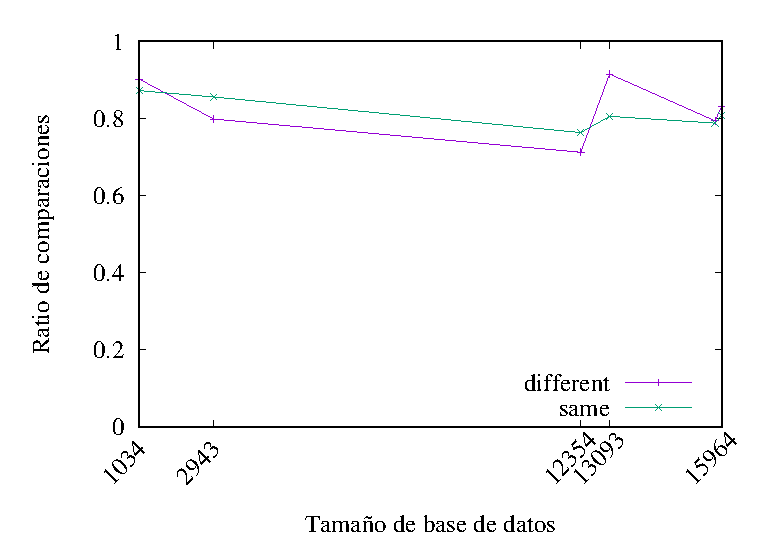
\includegraphics[width=71.5mm]{imagenes/same_vs_different/16p_incremental.eps}}
\subfigure[\scriptsize T\'ecnica de selecci\'on random]{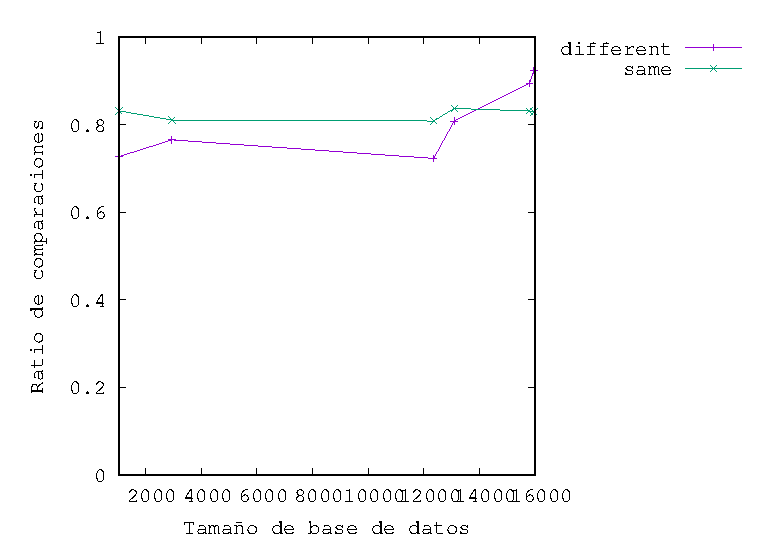
\includegraphics[width=71.5mm]{imagenes/same_vs_different/16p_random.eps}}
		\caption{\small Estrategia de selecci\'on para 16 pivotes: mismos pivotes vs diferentes}
		\label{fig:same-vs-diff-16Pivotes}
\end{figure}

\begin{figure}[H]
\centering
\subfigure[\scriptsize T\'ecnica de selecci\'on incremental]{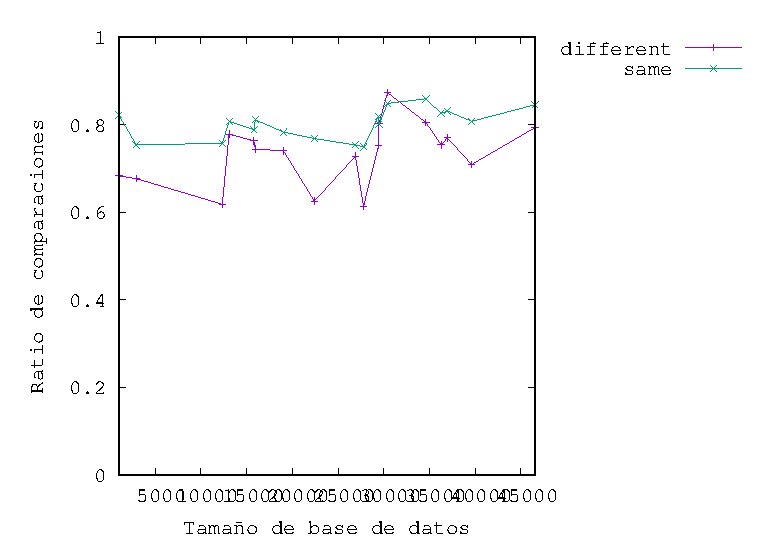
\includegraphics[width=71.5mm]{imagenes/same_vs_different/64p_incremental.eps}}
\subfigure[\scriptsize T\'ecnica de selecci\'on random]{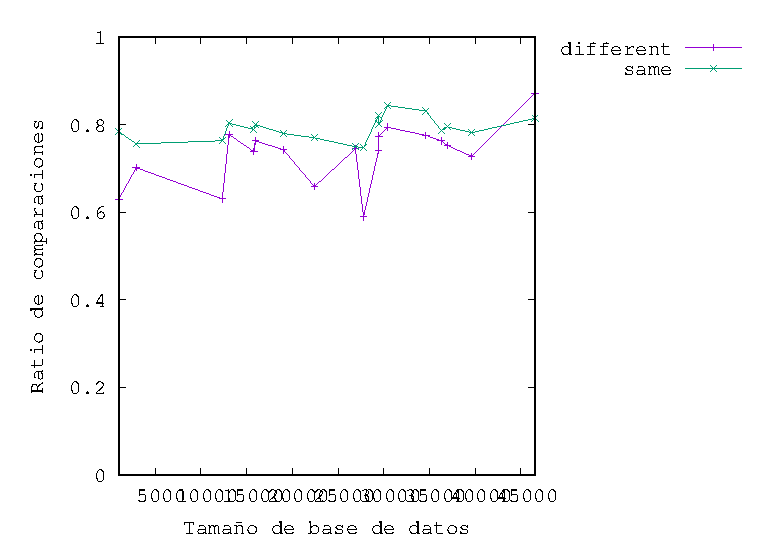
\includegraphics[width=71.5mm]{imagenes/same_vs_different/64p_random.eps}}
		\caption{\small Estrategia de selecci\'on para 64 pivotes: mismos pivotes vs diferentes}
		\label{fig:same-vs-diff-64Pivotes}
\end{figure}

%figuras comentadas
\begin{comment} 

\begin{figure}[H]
	\begin{center}
		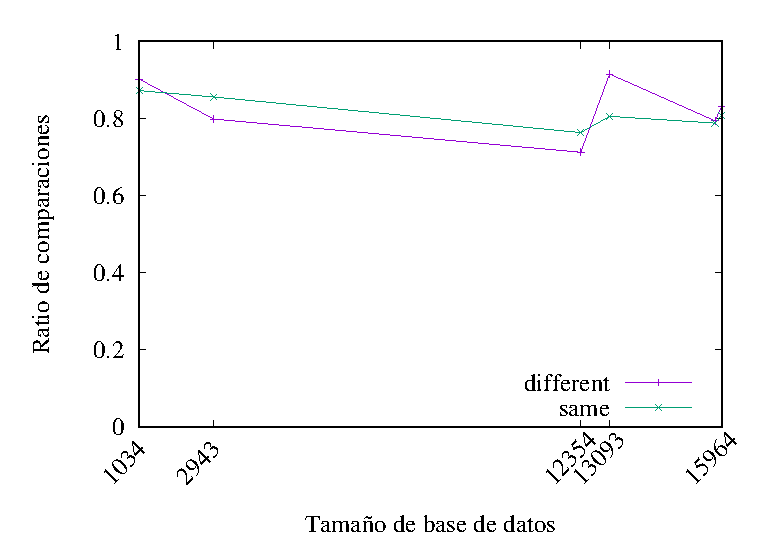
\includegraphics[width=1\textwidth]{imagenes/same_vs_different/16p_incremental.eps}
		\caption{\small Estrategia de selecci\'on incremental para 16 pivotes: mismos pivotes vs diferentes}
		\label{fig:same-vs-diff-Incremental-16Pivotes}

		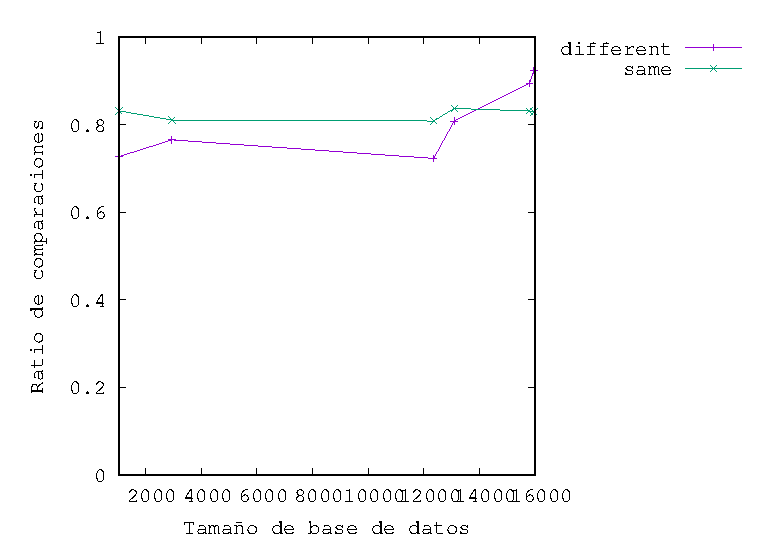
\includegraphics[width=1\textwidth]{imagenes/same_vs_different/16p_random.eps}
		\caption{\small Estrategia de selecci\'on random para 16 pivotes: mismos pivotes vs diferentes}
		\label{fig:same-vs-diff-random-16Pivotes}	

		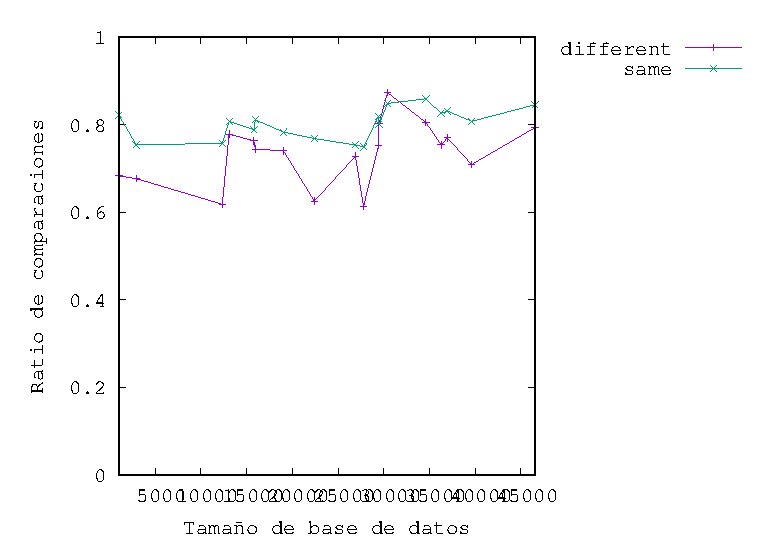
\includegraphics[width=1\textwidth]{imagenes/same_vs_different/64p_incremental.eps}
		\caption{\small Estrategia de selecci\'on incremental para 64 pivotes: mismos pivotes vs diferentes}
		\label{fig:same-vs-diff-Incremental-64Pivotes}
		
		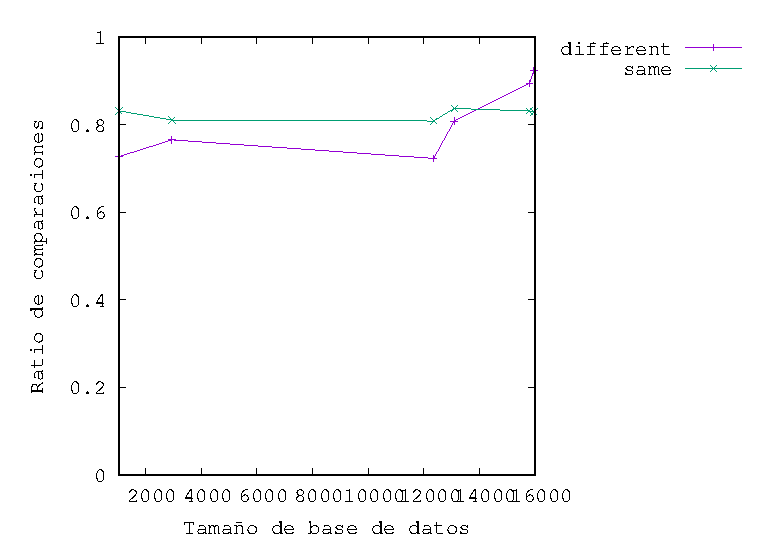
\includegraphics[width=1\textwidth]{imagenes/same_vs_different/16p_random.eps}
		\caption{\small Estrategia de selecci\'on random para 64 pivotes: mismos pivotes vs diferentes}
		\label{fig:same-vs-diff-random-64Pivotes}
	\end{center}
\end{figure}

\end{comment}

\section{Ejecuci\'on experimental}

En una segunda etapa,  nos concentramos en c\'omo agrupar los datos teniendo en cuenta la variaci\'on del tama\~no de las bases de datos para luego poder analizar la informaci\'on segmentada y poder sacar mejores conclusiones.\\

\subsection{Creaci\'on de grupos}

Dada la variabilidad de tamaños de las bases de datos, para poder analizar luego los resultados correctamente, definimos cuatro grupos segmentados por el tamaño de base de datos y por cantidad de pivotes. Esto es, calculamos el ratio de pivotes sobre el tamaño de las base de datos (DB), quedando la siguiente distribuci\'on:\\

\begin{table}[htbp]
\begin{center}
\begin{tabular}{|p{1.1cm}|p{1.8cm}|p{3.2cm}|p{2.2cm}|p{2.5cm}|}
\hline
Grupo & 
Cantidad de DB & 
Rango del tama\~no de DB & 
N\'umero de Pivotes &  
Cantidad de Experimentos\\
\hline \hline
1 & 
6 & 
[1.034 - 15.964] & 
16, 32, 64, 128, 256 & 
60  \\ \hline
2 &
12 &
[19.032 - 46.530] &
64, 128, 256, 512, 1024 &
120  \\ \hline
3 &
8 &
[57.198 - 13.6323] &
256, 512, 1024, 2048 &
64  \\ \hline
4 &
4 &
[16.7995- 21.3578] &
512, 1024, 2048, 4096 &
32  \\ \hline
\end{tabular}
\caption{Tabla de grupos.}
\label{tabla:grupos}
\end{center}
\end{table}

En total se ejecutaron 276 experimentos. Esto es, 138 experimentos usando t\'ecnica de selecci\'on de pivotes random y 138 experimentos usando t\'ecnica de selecci\'on de pivotes incremental.\\

Se seleccion\'o al azar el 10\% de los elementos de cada una de las bases de datos para realizar las b\'usquedas. La cantidad total de b\'usquedas por rango realizadas fue: 339.899. Este valor incluye las b\'usquedas usadas para descartar la pol\'itica de selecci\'on \textit{Mismo grupo de pivotes para todas las categor\'ias o bases de datos} mencionada anteriormente.\\

\section{An\'alisis de resultados}

Vamos a presentar los resultados segmentados en cuatro grupos y analizaremos tres enfoques diferentes.\\

Llamaremos ratio de comparaciones al porcentaje de comparaciones respecto del tamaño de la base de datos, esto es porcentaje de filtrado.\\

\subsection{Efecto de las t\'ecnicas de selecci\'on de pivotes}

En esta secci\'on vamos a comparar las t\'ecnicas de selecci\'on de pivotes random e incremental, usando como m\'etrica el n\'umero de evaluaciones de distancia para cada unos de los grupos de pivotes elegidos. Se realizaron las comparaciones para todas las bases de datos con las que trabajamos (30) pero a continuaci\'on s\'olo analizaremos la base de datos de mayor tama\~no de cada uno de los grupos que mencionamos anteriormente, el resto se adjuntan en el Anexo \ref{anexo.A}.\\

Para el grupo 1, figura \ref{fig:ETS-1}(a), observamos que para una base de datos de aproximadamente 16 mil elementos,  usando la t\'ecnica de selecci\'on incremental se realizan menos evaluaciones de distancia que la t\'ecnica de selecci\'on random para todos los grupos de pivotes, excepto para 128 pivotes. Tambi\'en se puede observar que la diferencia entre ambas t\'ecnicas es amplia.\\

Para el grupo 2, figura \ref{fig:ETS-1}(b), para una base de datos de aproximadamente 45 mil elementos, la t\'ecnica de selecci\'on incremental es mejor solo en dos grupos de pivotes, 64 y 256. Para los grupos de pivotes de 128, 512 y 1024, la t\'ecnica de selecci\'on random realiza menos evaluaciones de distancia que incremental. Tambi\'en se puede observar que a partir del grupo de pivotes 256, la diferencia de evaluaciones de distancia no es tan grande entre ambas t\'ecnicas.\\

Para el grupo 3, figura \ref{fig:ETS-2}(a), con una base de datos de aproximadamente 136 mil elementos, la t\'ecnica de selecci\'on incremental en general realiza menos cantidad de evaluaciones de distancia, salvo para 2048 pivotes. Para este ultimo grupo de pivotes, la t\'ecnica de selecci\'on random esta por debajo de incremental pero solo por muy poca diferencia.\\

Para el grupo 4, figura \ref{fig:ETS-2}(b), con una base de datos de aproximadamente 213 mil elementos, en general, la t\'ecnica de selecci\'on random, por muy poca diferencia (excepto para 4096, donde la diferencia es mas marcada), realiza menos cantidad de evaluaciones de distancia que la t\'ecnica de selecci\'on incremental.\\


\begin{figure}[H]
\centering
\subfigure[\scriptsize Grupo 1]{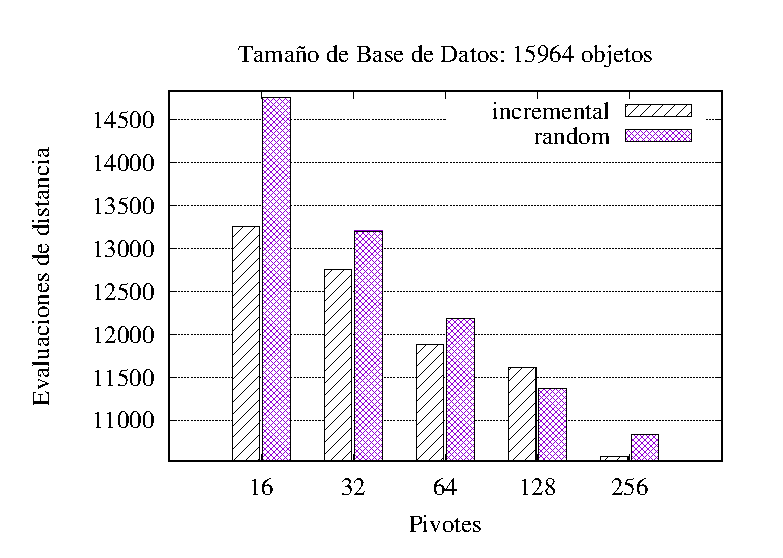
\includegraphics[width=71.5mm]{imagenes/random_vs_incremental/g1_15964.eps}}
\subfigure[\scriptsize Grupo 2]{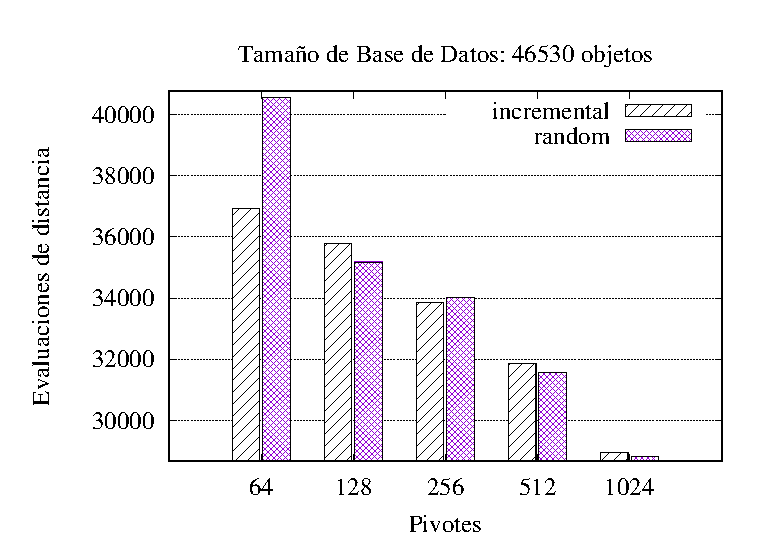
\includegraphics[width=71.5mm]{imagenes/random_vs_incremental/g2_46530.eps}}
\caption{\small Efecto de las t\'ecnicas de selecci\'on de pivotes random vs incremental respecto de evaluaciones de distancia.}
\label{fig:ETS-1}
\end{figure}
\begin{figure}[H]
\centering
\subfigure[\scriptsize Grupo 3]{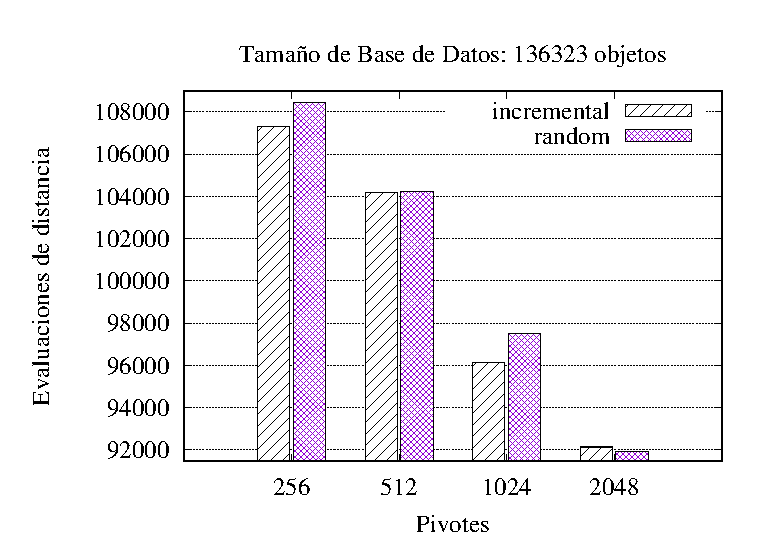
\includegraphics[width=71.5mm]{imagenes/random_vs_incremental/g3_136323.eps}}
\subfigure[\scriptsize Grupo 4]{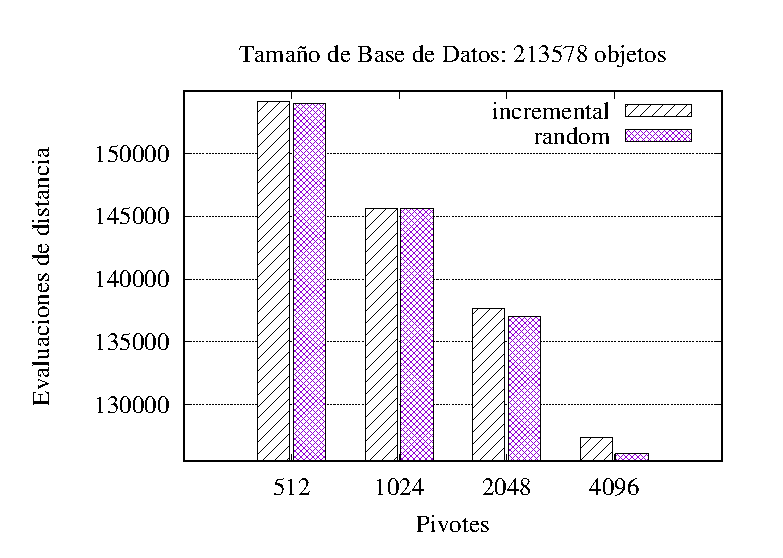
\includegraphics[width=71.5mm]{imagenes/random_vs_incremental/g4_213578.eps}}
\caption{\small Efecto de las t\'ecnicas de selecci\'on de pivotes random vs incremental respecto de evaluaciones de distancia.}
\label{fig:ETS-2}

\end{figure}

Como conclusi\'on general, se puede observar que la t\'ecnica de selecci\'on random realiza menos cantidad de evaluaciones de distancia, aunque por muy poca diferencia.\\
 
Dado que el comportamiento para ambas t\'ecnicas de selecci\'on no era el que esperabamos, es decir, incremental no era mucho mejor que random en cuanto a ratio de comparaciones, hicimos un an\'alisis emp\'irico sobre diferentes categor\'ias para entender tal comportamiento. Este an\'alisis lo veremos mas adelante en detalle.

\subsection{Efecto de la cantidad de pivotes}

A continuaci\'on vamos a analizar el efecto de la cantidad de pivotes sobre el ratio de comparaciones para cada base de datos. Cada l\'ineas representa una base de datos y estas bases de datos est\'an representadas por su tamaño como se muestra en las gr\'aficas.\\

En la figura \ref{fig:EP-g1}, observamos que tanto para selecci\'on de pivotes random (a) como para selecci\'on de pivotes incremental (b), para $16, 32, 64, 128$ y $256$ pivotes, a media que aumenta el n\'umero de pivotes el ratio de comparaciones disminuye. Tambi\'en vemos que las 3 bases de datos mas grandes, tienen un comportamiento similar, es decir el ratio de comparaciones oscila entre $0,7$ y $0,93$ aproximadamente y para las 3 bases de datos mas chicas, oscila entre $0,4$ y $0,8$ aproximadamente.\\

En la figura \ref{fig:EP-g2}, observamos que para los pivotes $64, 128, 256, 512$ y $1024$ ambas t\'ecnicas de selecci\'on de pivotes se comportan semejantes, a mayor n\'umero de pivotes menor ratio de comparaciones. El ratio de comparaciones est\'a entre $0,6$ y $0,8$ para todas las bases de datos excepto la $27788$ que se encuentra entre $0,4$ y $0,6$.\\

En la figura \ref{fig:EP-g3}, observamos el mismo comportamiento que para los grupos 1 y 2 mencionados anteriormente. En ambas t\'ecnicas de selecci\'on de pivotes, para la mayor\'ia de las bases de datos el ratio de comparaciones est\'a entre $0,6$ y $0,8$. Para pivotes de este grupo, $256, 512, 1024$ y $2048$, tambi\'en, a mayor n\'umero de pivotes menor ratio de comparaciones.\\

En la figura \ref{fig:EP-g4}, observamos que a media que aumenta el n\'umero de pivotes el ratio de comparaciones disminuye, similar al resto de los grupos. Tambi\'en vemos que 3 de las 4 bases de datos que estamos analizando, para los pivotes 512, 1024 y 2048; el ratio de comparaciones esta entre $0,6$ y $0,75$ aproximadamente y para 4096 pivotes, entre $0,5$ $0,6$.\\

A modo de resumen, analizando el efecto de la cantidad de pivotes en general para los cuatro grupos, vemos que cuando aumenta el n\'umero de pivotes se decrementa el ratio de comparaciones pero las t\'ecnicas de selecci\'on random e incremental, no muestran diferencias entre ellas.

\begin{figure}[H]
\centering
\subfigure[\scriptsize T\'ecnica de selecci\'on de pivotes random]{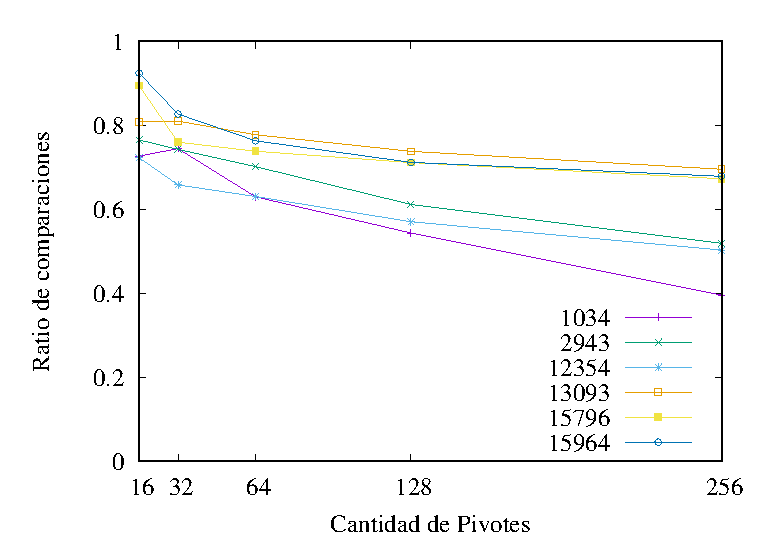
\includegraphics[width=71.5mm]{imagenes/efecto_pivotes/g1_random_ep.eps}}
\subfigure[\scriptsize T\'ecnica de selecci\'on de pivotes incremental]{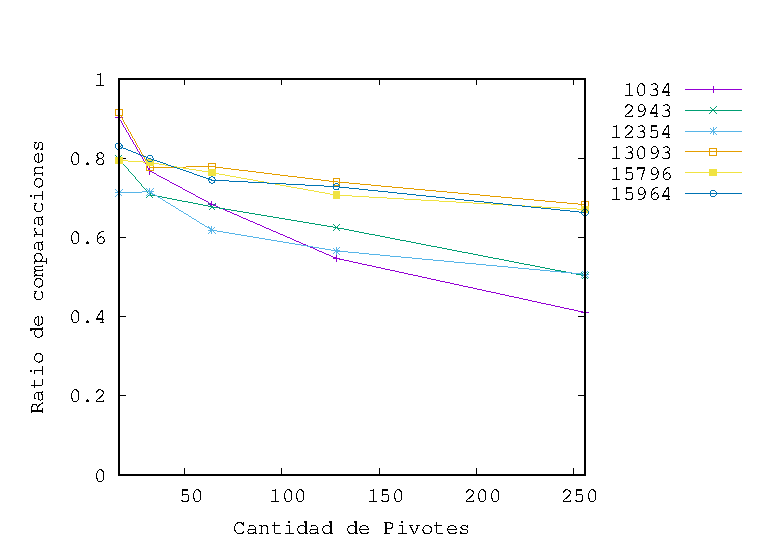
\includegraphics[width=71.5mm]{imagenes/efecto_pivotes/g1_incremental_ep.eps}}
		\caption{\small Grupo 1 - Efecto de la cantidad de pivotes sobre el ratio de comparaciones.}
		\label{fig:EP-g1}
\end{figure}

\begin{figure}[H]
\centering
\subfigure[\scriptsize T\'ecnica de selecci\'on de pivotes random]{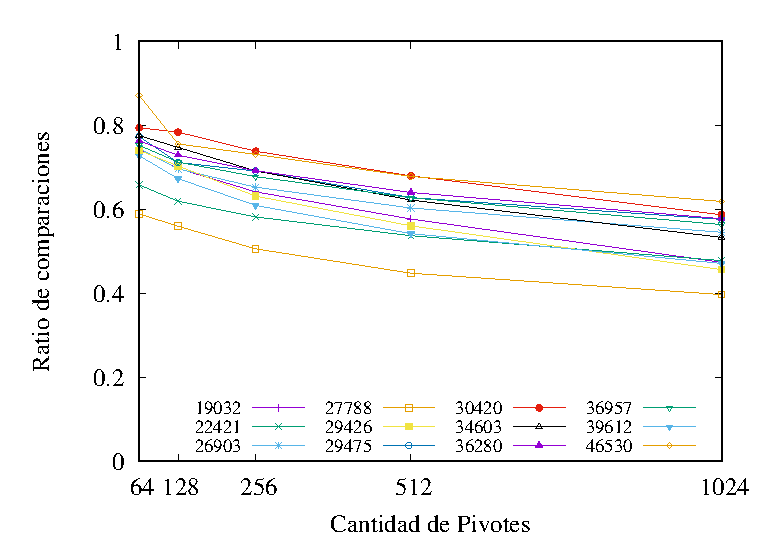
\includegraphics[width=71.5mm]{imagenes/efecto_pivotes/g2_random_ep.eps}}
\subfigure[\scriptsize T\'ecnica de selecci\'on de pivotes incremental]{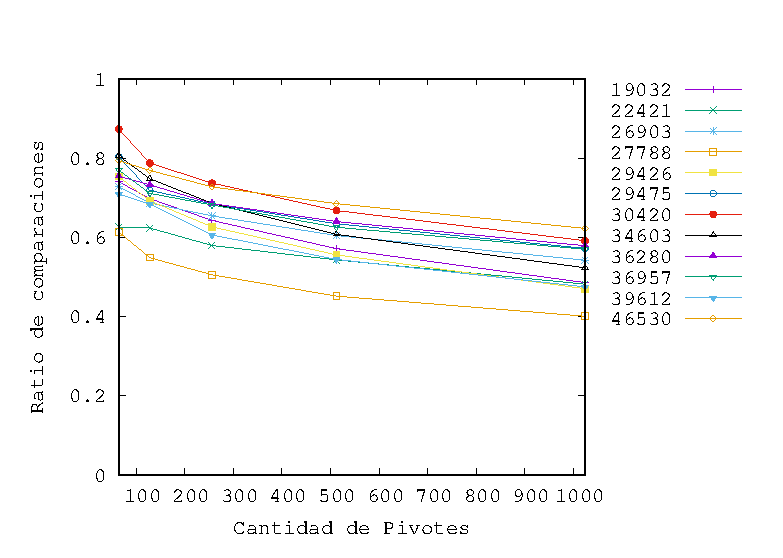
\includegraphics[width=71.5mm]{imagenes/efecto_pivotes/g2_incremental_ep.eps}}
		\caption{\small Grupo 2 - Efecto de la cantidad de pivotes sobre el ratio de comparaciones.}
		\label{fig:EP-g2}
\end{figure}

\begin{figure}[H]
\centering
\subfigure[\scriptsize T\'ecnica de selecci\'on de pivotes random]{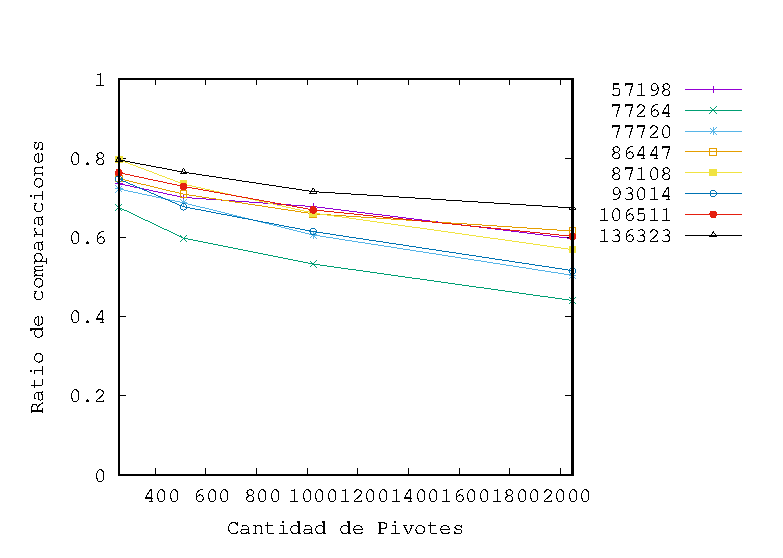
\includegraphics[width=71.5mm]{imagenes/efecto_pivotes/g3_random_ep.eps}}
\subfigure[\scriptsize T\'ecnica de selecci\'on de pivotes incremental]{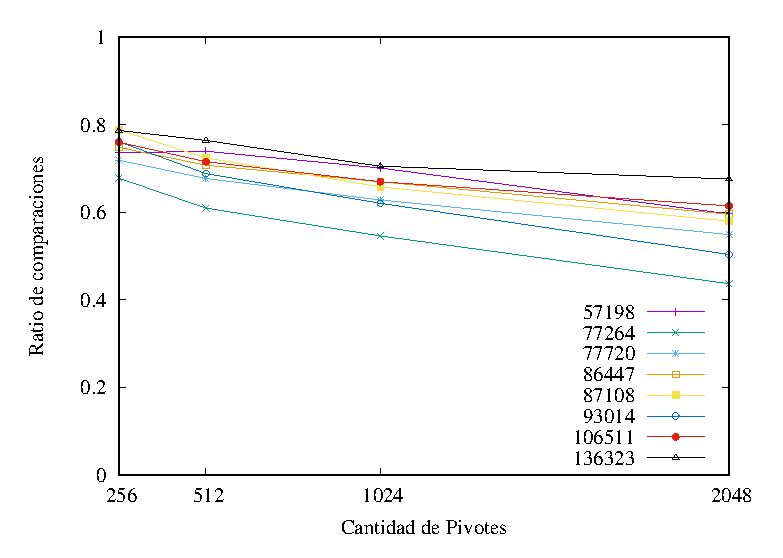
\includegraphics[width=71.5mm]{imagenes/efecto_pivotes/g3_incremental_ep.eps}}
		\caption{\small Grupo 3 - Efecto de la cantidad de pivotes sobre el ratio de comparaciones.}
		\label{fig:EP-g3}
\end{figure}

\begin{figure}[H]
\centering	
\subfigure[\scriptsize T\'ecnica de selecci\'on de pivotes random]{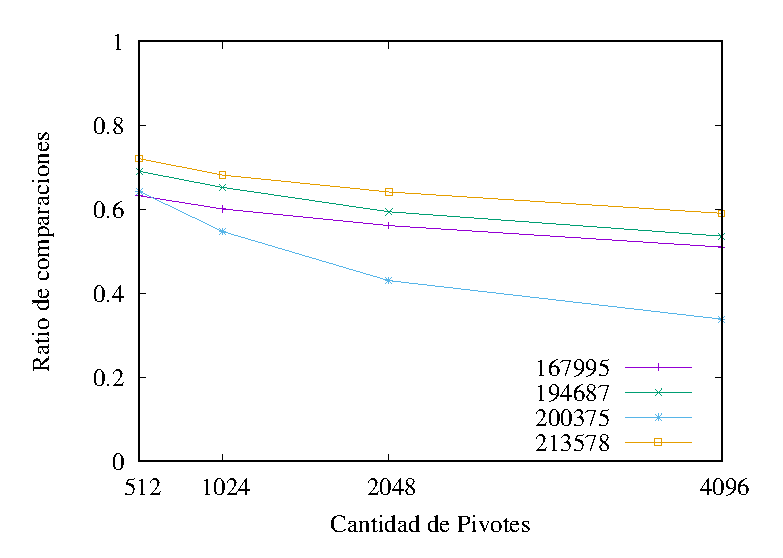
\includegraphics[width=71.5mm]{imagenes/efecto_pivotes/g4_random_ep.eps}}
\subfigure[\scriptsize T\'ecnica de selecci\'on de pivotes incremental]{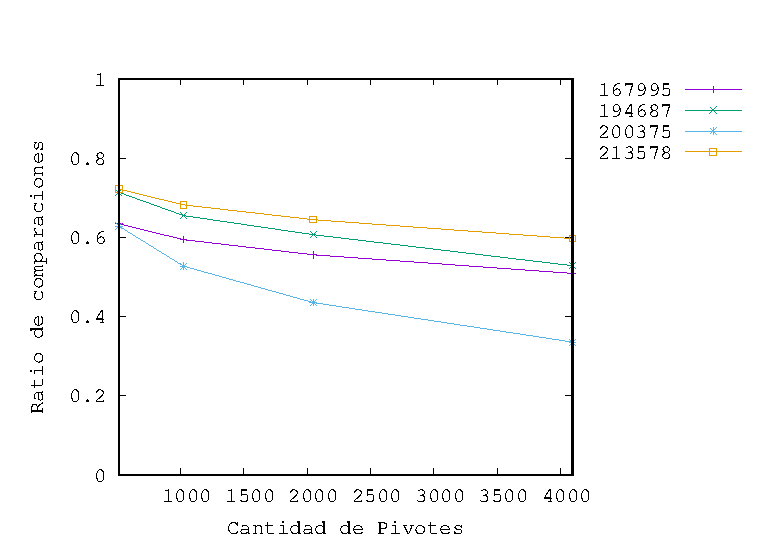
\includegraphics[width=71.5mm]{imagenes/efecto_pivotes/g4_incremental_ep.eps}}
		\caption{\small Grupo 4 - Efecto de la cantidad de pivotes sobre el ratio de comparaciones.}
		\label{fig:EP-g4}
\end{figure}

\subsection{Efecto tamaño de la base de datos}

A continuaci\'on vamos a analizar cual es el efecto del tama\~no de las bases de datos sobre el ratio de comparaciones por pivotes. Las l\'ineas de las graficas son el n\'umero de pivotes con los que se ejecutaron las b\'usquedas.\\

En la figura \ref{fig:EDB-g1} tenemos el grupo 1; donde el rango del tama\~no de las bases de datos es $[1.034-15.964]$ y los pivotes usados son $16, 32, 64, 128$ y $256$. Para la t\'ecnica de selecci\'on de pivotes random (a), en la base de datos mas chica, el ratio de comparaciones esta entre $0,4$ y $0,8$ y para las base de datos m\'as grandes, entre $0,7$ y $0,9$. Por otro lado, si miramos la gr\'afica para $256$ pivotes podemos observar que para las base de datos mas chica el ratio de comparaciones es $0,4$ y a medida que crece en tama\~no de la base de datos el ratio de comparaciones tambien aumenta ($0,7$ en las bases de datos mas grandes).\
Para la t\'ecnica de selecci\'on de pivotes incremental (b), el comportamiento es similar, a menor cantidad de pivotes, mayor ratio de comparaciones.\\

En la figura \ref{fig:EDB-g2}, donde el tama\~no de las bases de datos van desde $19032$ a $46530$ elementos y los pivotes usados son $64, 128, 256, 512$ y $1024$, el ratio de comparaciones no tiene mucha variabilidad desde la base de datos mas chica a las mas grande.\
Por ejemplo: para t\'ecnica de selecci\'on de pivotes random, 512 pivotes y una bade de datos de 19 mil elementos el ratio de comparaciones es $0,58$ aproximadamente y para una base de datos de 46 mil elementos, el ratio es $0,67$. Estos valores son similares para el caso de t\'ecnica de selecci\'on de pivotes incremental.\
A nivel general, para t\'ecnica de selecci\'on de pivotes random, podemos ver que para la base de datos mas chica, el ratio de comparaciones varia entre 0,49 y 0,79; y para las base de datos mas grande, entre 0,6 y 0,84. Para t\'ecnica de selecci\'on de pivotes incremental los rangos de ratios de comparaciones estan entre $[0,5 - 0,77]$ y $[0,61 - 0,79]$. \\

Para las figuras \ref{fig:EDB-g3} y \ref{fig:EDB-g4}, donde se muestran los grupos 3 y 4 respectivamente, el comportamiento es similar al de los grupos antes mencionados.	\
A medida que el tama\~no de las base de datos aumenta, el ratio de comparaciones tambi\'en crece, aunque la variabilidad de este \'ultimo es muy baja. Esto es similiar en ambas  t\'ecnica de selecci\'on de pivotes.

\begin{figure}[H]
\centering
\subfigure[\scriptsize T\'ecnica de selecci\'on de pivotes random]{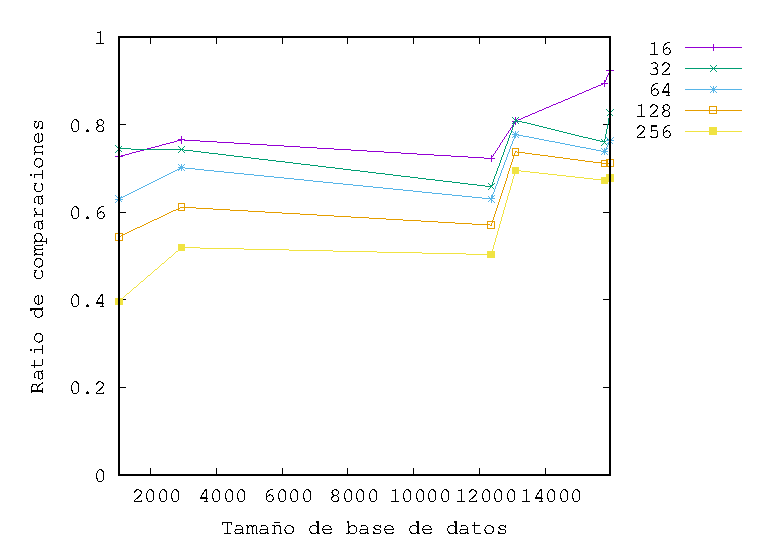
\includegraphics[width=71.5mm]{imagenes/efecto_db/g1_random_edb.eps}}
\subfigure[\scriptsize T\'ecnica de selecci\'on de pivotes incremental]{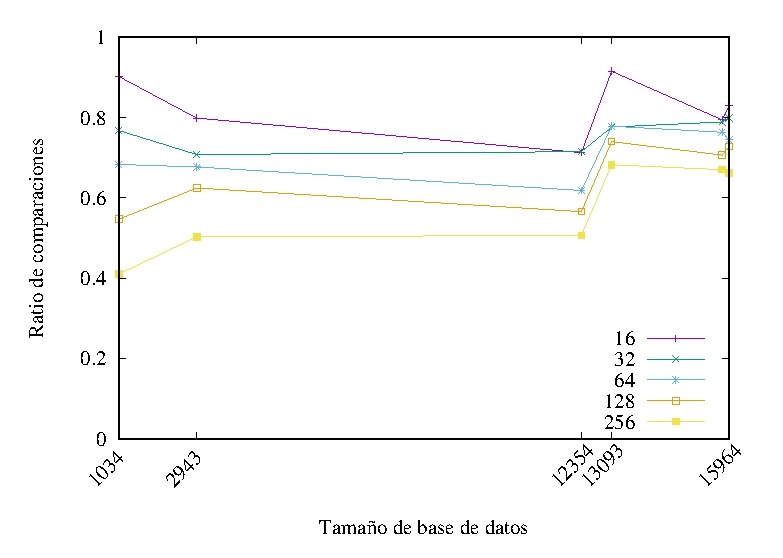
\includegraphics[width=71.5mm]{imagenes/efecto_db/g1_incremental_edb.eps}}
		\caption{\small Grupo 1 - Efecto del tamaño de la base de datos sobre el ratio de comparaciones por pivotes.}
		\label{fig:EDB-g1}
\subfigure[\scriptsize T\'ecnica de selecci\'on de pivotes random]{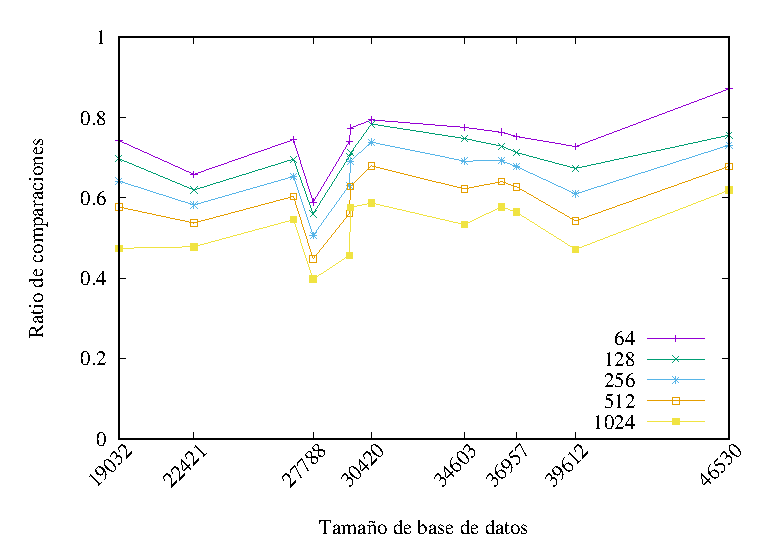
\includegraphics[width=71.5mm]{imagenes/efecto_db/g2_random_edb.eps}}
\subfigure[\scriptsize T\'ecnica de selecci\'on de pivotes incremental]{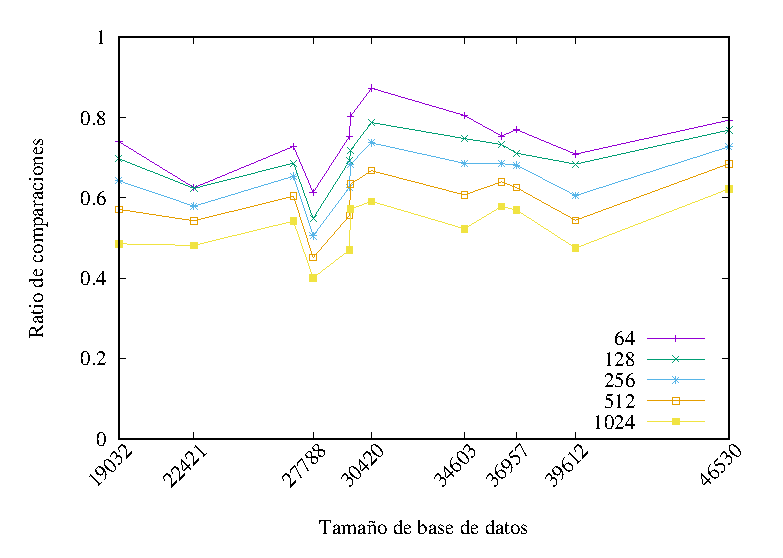
\includegraphics[width=71.5mm]{imagenes/efecto_db/g2_incremental_edb.eps}}
		\caption{\small Grupo 2 - Efecto del tamaño de la base de datos sobre el ratio de comparaciones por pivotes.}
		\label{fig:EDB-g2}
\subfigure[\scriptsize T\'ecnica de selecci\'on de pivotes random]{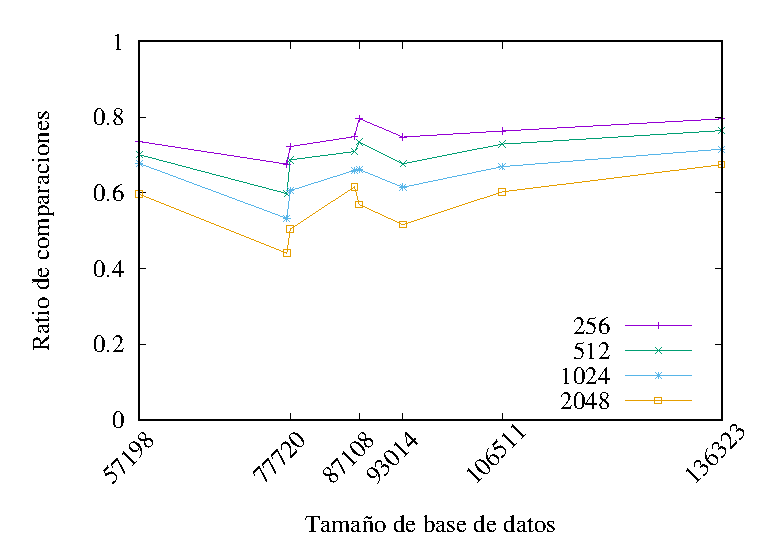
\includegraphics[width=71.5mm]{imagenes/efecto_db/g3_random_edb.eps}}
\subfigure[\scriptsize T\'ecnica de selecci\'on de pivotes incremental]{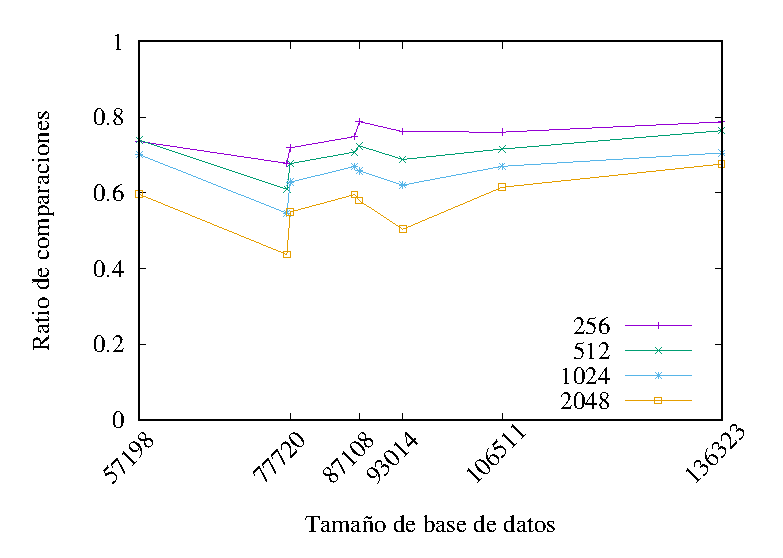
\includegraphics[width=71.5mm]{imagenes/efecto_db/g3_incremental_edb.eps}}
		\caption{\small Grupo 3 - Efecto del tamaño de la base de datos sobre el ratio de comparaciones por pivotes.}
		\label{fig:EDB-g3}
\end{figure}

\begin{figure}[H]
\centering
\subfigure[\scriptsize T\'ecnica de selecci\'on de pivotes random]{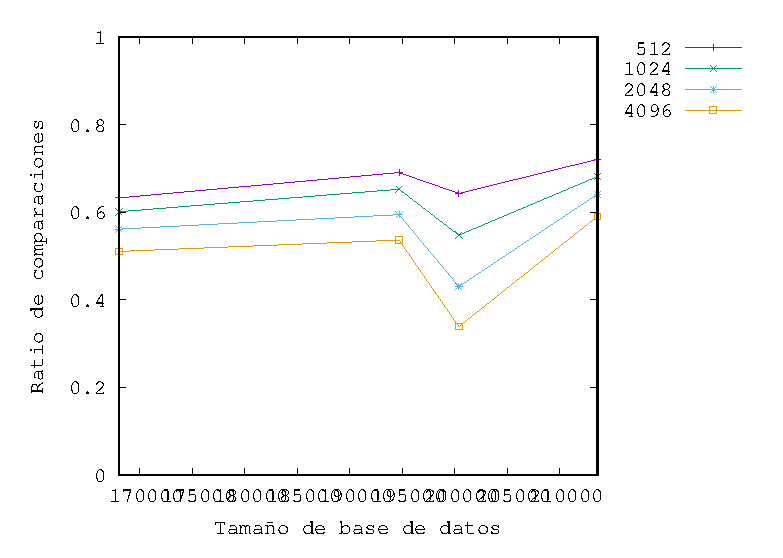
\includegraphics[width=71.5mm]{imagenes/efecto_db/g4_random_edb.eps}}
\subfigure[\scriptsize T\'ecnica de selecci\'on de pivotes incremental]{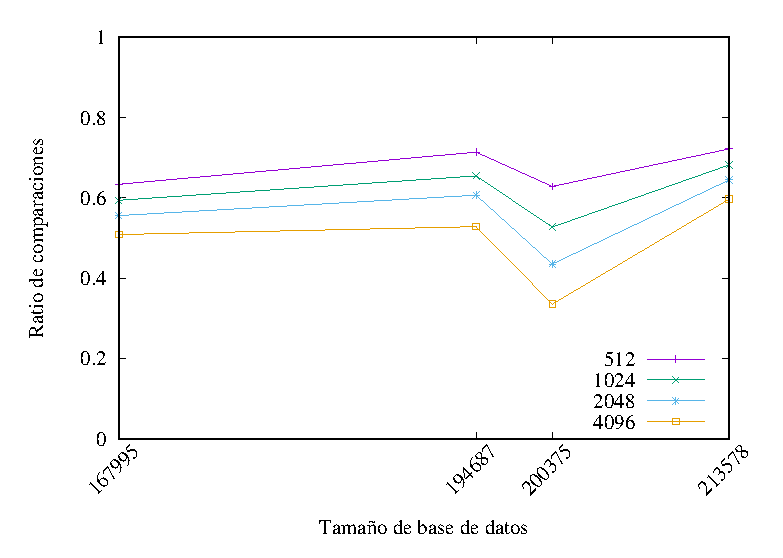
\includegraphics[width=71.5mm]{imagenes/efecto_db/g4_incremental_edb.eps}}
		\caption{\small Grupo 4 - Efecto del tamaño de la base de datos sobre el ratio de comparaciones por pivotes.}
		\label{fig:EDB-g4}
\end{figure}
 
